\lab{Applications}{RiverCrossing}{RiverCrossing}
\label{lab:rivercrossing}
\objective{Introductory lab discussing a classical calculus of variations problem: how is a river to be crossed in the shortest possible time? We will look at a numerical solution using the pseudospectral method. }


Suppose that the graph of a function $y(x), \, x\in [-1,1]$ describes the path of a boat as it crosses a river. We assume that the speed at which the boat is rowed remains constant. The time required for the boat to cross the river can be described by the functional 
\begin{align*}
T[y] &=  \int_{-1}^1 L(x,y,y')\, dx
% \int_{-1}^1 a(x) \sqrt{1 + a^2(x)(y'(x))^2} - a^2(x)r(x)y'(x)\, dx 
\end{align*}
where 
\begin{align*}
	L(x,y,y') &= \alpha(x) \sqrt{1 + \alpha^2(x)(y')^2} - \alpha^2(x)c(x)y', \\
	\alpha(x) &= (1-c^2(x))^{-1/2},
\end{align*}
and $c(x)$ is a known function that describes the current of the river at any point $x \in [-1,1]$. We will assume that the current is faster near the center of the river. 




We look for the path $y(x)$ that minimizes the time required for the boat to cross the river, so that the function $T$ is minimized. From the calculus of variations we know that a smooth path $y(x)$ minimizes $T$ only if the Euler-Lagrange equation is satisfied. Recall that the Euler-Lagrange equation is 
\[
% \frac{\partial }{\partial y}L - \frac{d}{dx}\frac{\partial }{\partial y'}L
L_{y} - \frac{d}{dx}L_{y'} = 0.
\]
Since $L_y = 0,$ this problem is equivalent to solving the first order ordinary differential equation
\begin{align*}
	L_{y'} = \alpha(x)(1 + \alpha^2 (y')^2)^{-1/2}\alpha^2 y' - \alpha^2 r =   k,
\end{align*}
where $k$ is some appropriately chosen constant. To help us choose integration constants, we will impose boundary conditions $y(-1) = 0$, $y(1) = y_1$. 



\begin{problem}
	Assume that $c(x)$ is given by $c(x) = -.5(x-1)(x+1)$.%, and $y(1) = y_1$.
	Write a Python function that accepts as arguments a function $y$ (or $y'$) and an $x$-value, and returns $L(x,y(x),y'(x))$. Use that function to define a second function that numerically computes $T[y]$ for a given path $y(x)$.
\end{problem}



\begin{figure}
\centering
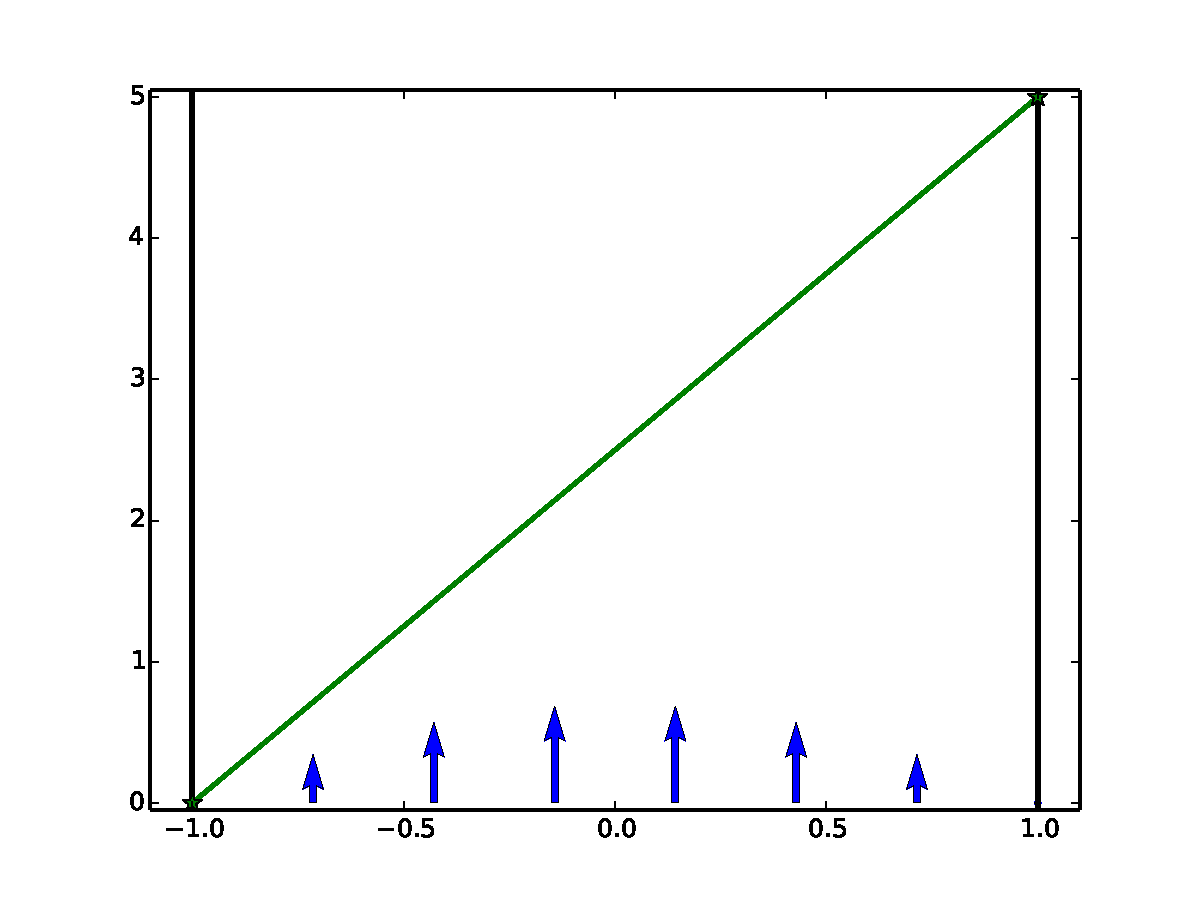
\includegraphics[width=\textwidth]{rivercurrent.pdf}
\caption{We will use the function $c(x) = -.5(x-1)(x+1)$ to describe the river's current.}
\label{fig:rivercrossing_current}
\end{figure}







